\section{SceneGraphTest.cpp File Reference}
\label{SceneGraphTest_8cpp}\index{SceneGraphTest.cpp@{SceneGraphTest.cpp}}


{\tt \#include \char`\"{}stdafx.h\char`\"{}}\par
{\tt \#include $<$boost/test/auto\_\-unit\_\-test.hpp$>$}\par
{\tt \#include \char`\"{}GroupNode.h\char`\"{}}\par
{\tt \#include \char`\"{}SceneGraph.h\char`\"{}}\par
{\tt \#include $<$boost/shared\_\-ptr.hpp$>$}\par
{\tt \#include $<$iostream$>$}\par
{\tt \#include \char`\"{}ListGraphVisitor.h\char`\"{}}\par


Include dependency graph for SceneGraphTest.cpp:\nopagebreak
\begin{figure}[H]
\begin{center}
\leavevmode
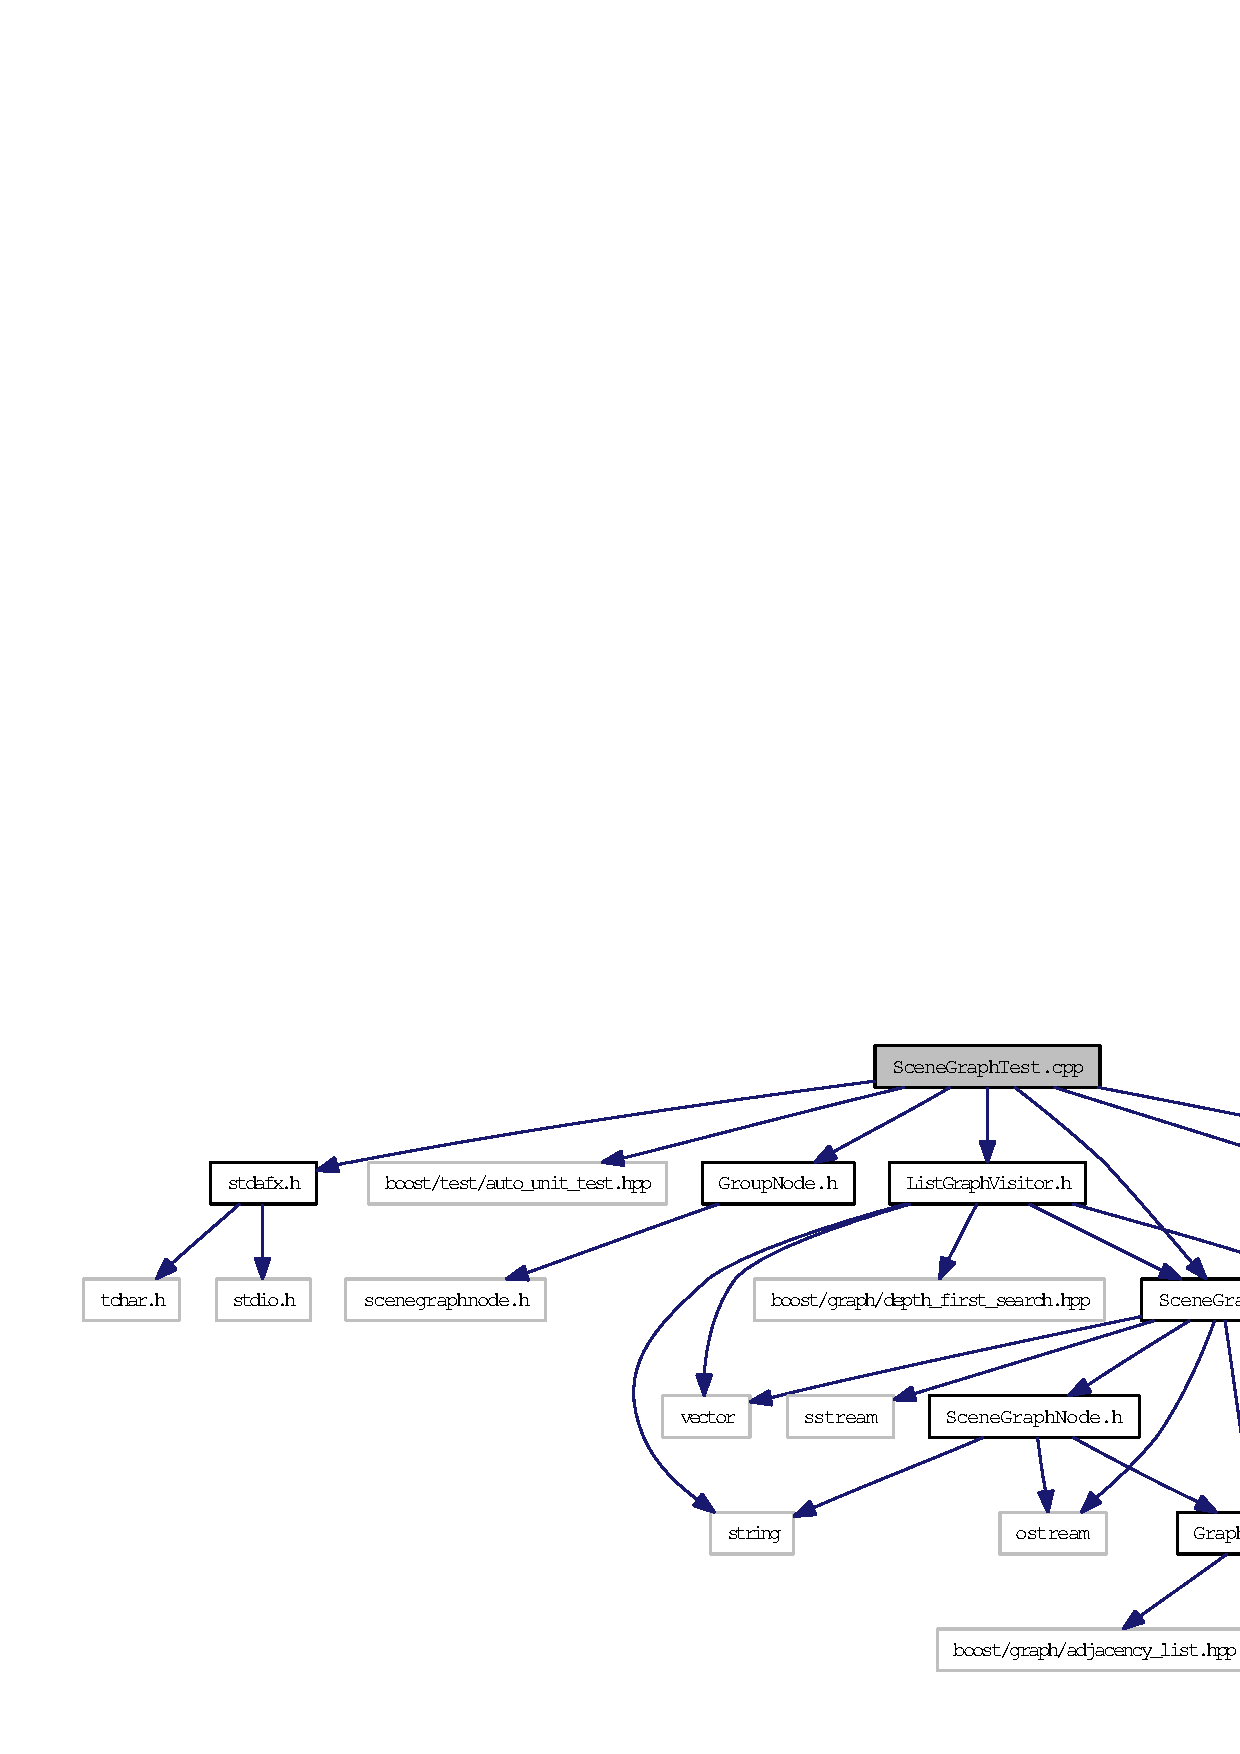
\includegraphics[width=420pt]{SceneGraphTest_8cpp__incl}
\end{center}
\end{figure}
\subsection*{Defines}
\begin{CompactItemize}
\item 
\#define {\bf BOOST\_\-AUTO\_\-TEST\_\-MAIN}
\end{CompactItemize}
\subsection*{Functions}
\begin{CompactItemize}
\item 
{\bf BOOST\_\-AUTO\_\-TEST\_\-CASE} (scene\_\-graph\_\-stream\_\-operator\_\-test)
\item 
{\bf BOOST\_\-AUTO\_\-TEST\_\-CASE} (scene\_\-graph\_\-add\_\-root\_\-node\_\-test)
\item 
{\bf BOOST\_\-AUTO\_\-TEST\_\-CASE} (scene\_\-graph\_\-add\_\-node\_\-test)
\item 
{\bf BOOST\_\-AUTO\_\-TEST\_\-CASE} (print\_\-vertices\_\-test)
\item 
{\bf BOOST\_\-AUTO\_\-TEST\_\-CASE} (pretty\_\-print\_\-vertices\_\-test)
\item 
{\bf BOOST\_\-AUTO\_\-TEST\_\-CASE} (write\_\-dot\_\-test)
\end{CompactItemize}


\subsection{Define Documentation}
\index{SceneGraphTest.cpp@{SceneGraphTest.cpp}!BOOST\_\-AUTO\_\-TEST\_\-MAIN@{BOOST\_\-AUTO\_\-TEST\_\-MAIN}}
\index{BOOST\_\-AUTO\_\-TEST\_\-MAIN@{BOOST\_\-AUTO\_\-TEST\_\-MAIN}!SceneGraphTest.cpp@{SceneGraphTest.cpp}}
\subsubsection{\setlength{\rightskip}{0pt plus 5cm}\#define BOOST\_\-AUTO\_\-TEST\_\-MAIN}\label{SceneGraphTest_8cpp_f00c3bd56a2dfa707b0534a7e1670af4}




Definition at line 5 of file SceneGraphTest.cpp.

\subsection{Function Documentation}
\index{SceneGraphTest.cpp@{SceneGraphTest.cpp}!BOOST\_\-AUTO\_\-TEST\_\-CASE@{BOOST\_\-AUTO\_\-TEST\_\-CASE}}
\index{BOOST\_\-AUTO\_\-TEST\_\-CASE@{BOOST\_\-AUTO\_\-TEST\_\-CASE}!SceneGraphTest.cpp@{SceneGraphTest.cpp}}
\subsubsection{\setlength{\rightskip}{0pt plus 5cm}BOOST\_\-AUTO\_\-TEST\_\-CASE (scene\_\-graph\_\-stream\_\-operator\_\-test)}\label{SceneGraphTest_8cpp_695bba67b053a15614907b5a5a9865f4}




Definition at line 14 of file SceneGraphTest.cpp.\index{SceneGraphTest.cpp@{SceneGraphTest.cpp}!BOOST\_\-AUTO\_\-TEST\_\-CASE@{BOOST\_\-AUTO\_\-TEST\_\-CASE}}
\index{BOOST\_\-AUTO\_\-TEST\_\-CASE@{BOOST\_\-AUTO\_\-TEST\_\-CASE}!SceneGraphTest.cpp@{SceneGraphTest.cpp}}
\subsubsection{\setlength{\rightskip}{0pt plus 5cm}BOOST\_\-AUTO\_\-TEST\_\-CASE (scene\_\-graph\_\-add\_\-root\_\-node\_\-test)}\label{SceneGraphTest_8cpp_ff59ac710519488fcf0379d712d8ef70}




Definition at line 24 of file SceneGraphTest.cpp.

References SceneGraph::addRootNode(), and SceneGraph::getNode().

Here is the call graph for this function:\nopagebreak
\begin{figure}[H]
\begin{center}
\leavevmode
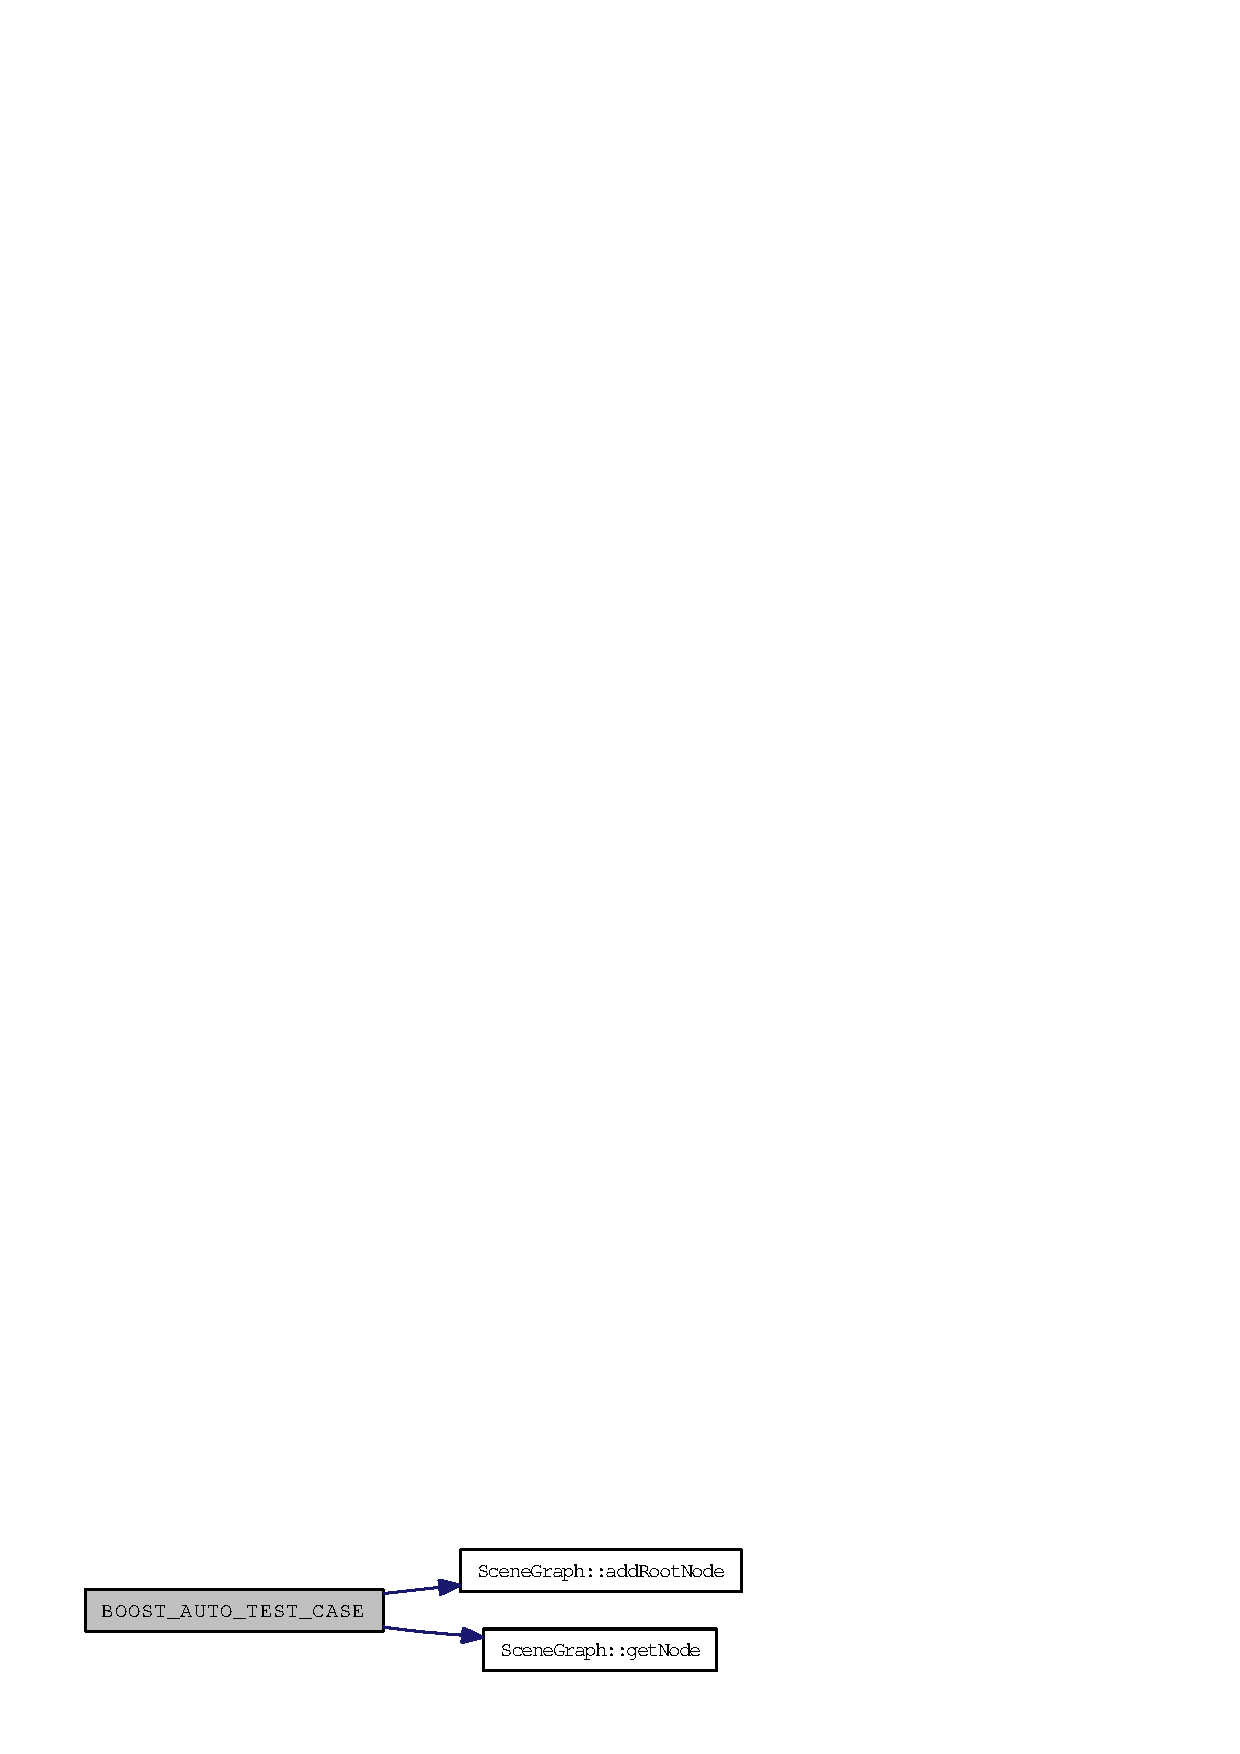
\includegraphics[width=180pt]{SceneGraphTest_8cpp_ff59ac710519488fcf0379d712d8ef70_cgraph}
\end{center}
\end{figure}
\index{SceneGraphTest.cpp@{SceneGraphTest.cpp}!BOOST\_\-AUTO\_\-TEST\_\-CASE@{BOOST\_\-AUTO\_\-TEST\_\-CASE}}
\index{BOOST\_\-AUTO\_\-TEST\_\-CASE@{BOOST\_\-AUTO\_\-TEST\_\-CASE}!SceneGraphTest.cpp@{SceneGraphTest.cpp}}
\subsubsection{\setlength{\rightskip}{0pt plus 5cm}BOOST\_\-AUTO\_\-TEST\_\-CASE (scene\_\-graph\_\-add\_\-node\_\-test)}\label{SceneGraphTest_8cpp_df69b1bb16fd0ae812e51c9ef665e5da}




Definition at line 34 of file SceneGraphTest.cpp.

References SceneGraph::addNode(), and SceneGraph::addRootNode().

Here is the call graph for this function:\nopagebreak
\begin{figure}[H]
\begin{center}
\leavevmode
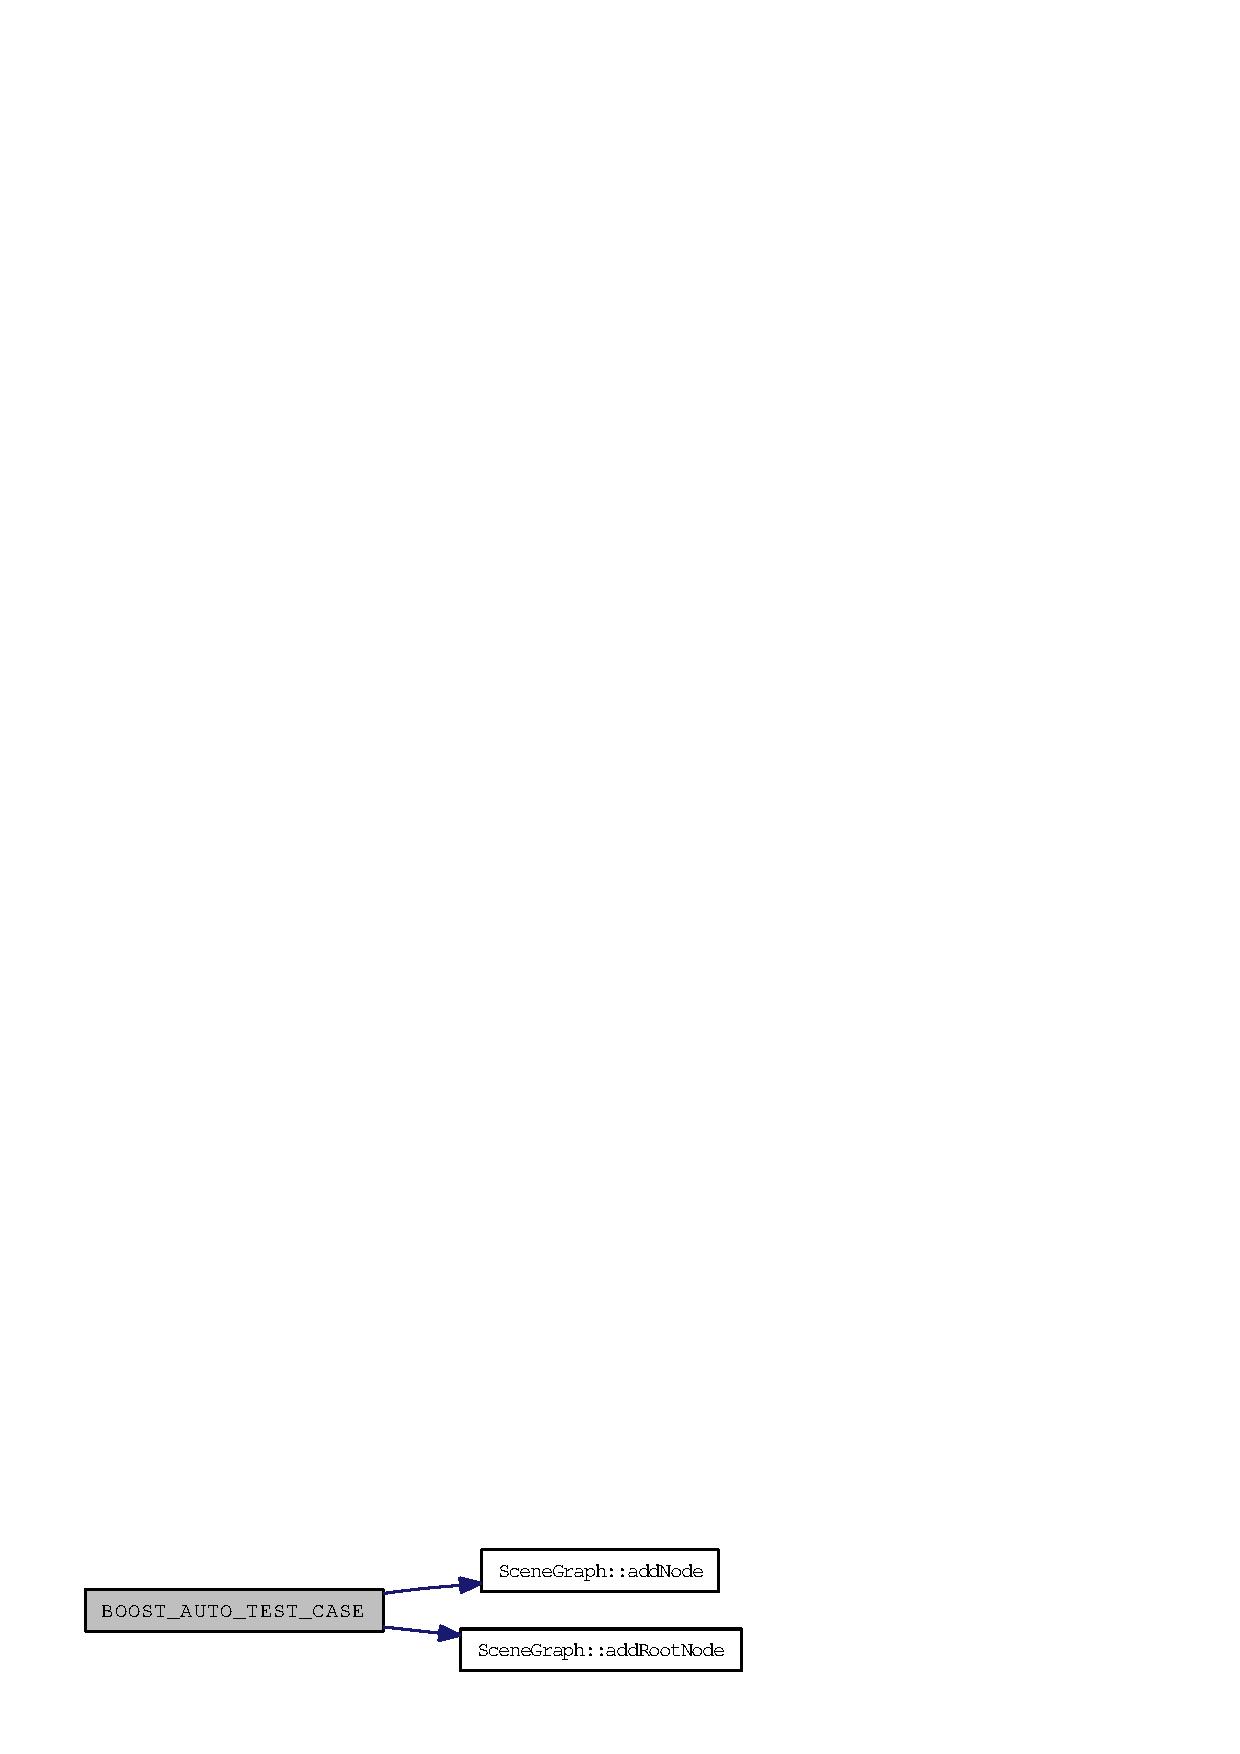
\includegraphics[width=180pt]{SceneGraphTest_8cpp_df69b1bb16fd0ae812e51c9ef665e5da_cgraph}
\end{center}
\end{figure}
\index{SceneGraphTest.cpp@{SceneGraphTest.cpp}!BOOST\_\-AUTO\_\-TEST\_\-CASE@{BOOST\_\-AUTO\_\-TEST\_\-CASE}}
\index{BOOST\_\-AUTO\_\-TEST\_\-CASE@{BOOST\_\-AUTO\_\-TEST\_\-CASE}!SceneGraphTest.cpp@{SceneGraphTest.cpp}}
\subsubsection{\setlength{\rightskip}{0pt plus 5cm}BOOST\_\-AUTO\_\-TEST\_\-CASE (print\_\-vertices\_\-test)}\label{SceneGraphTest_8cpp_950a30b389f81084f419f5614cef9808}




Definition at line 46 of file SceneGraphTest.cpp.

References SceneGraph::addNode(), SceneGraph::addRootNode(), and SceneGraph::listNodes().

Here is the call graph for this function:\nopagebreak
\begin{figure}[H]
\begin{center}
\leavevmode
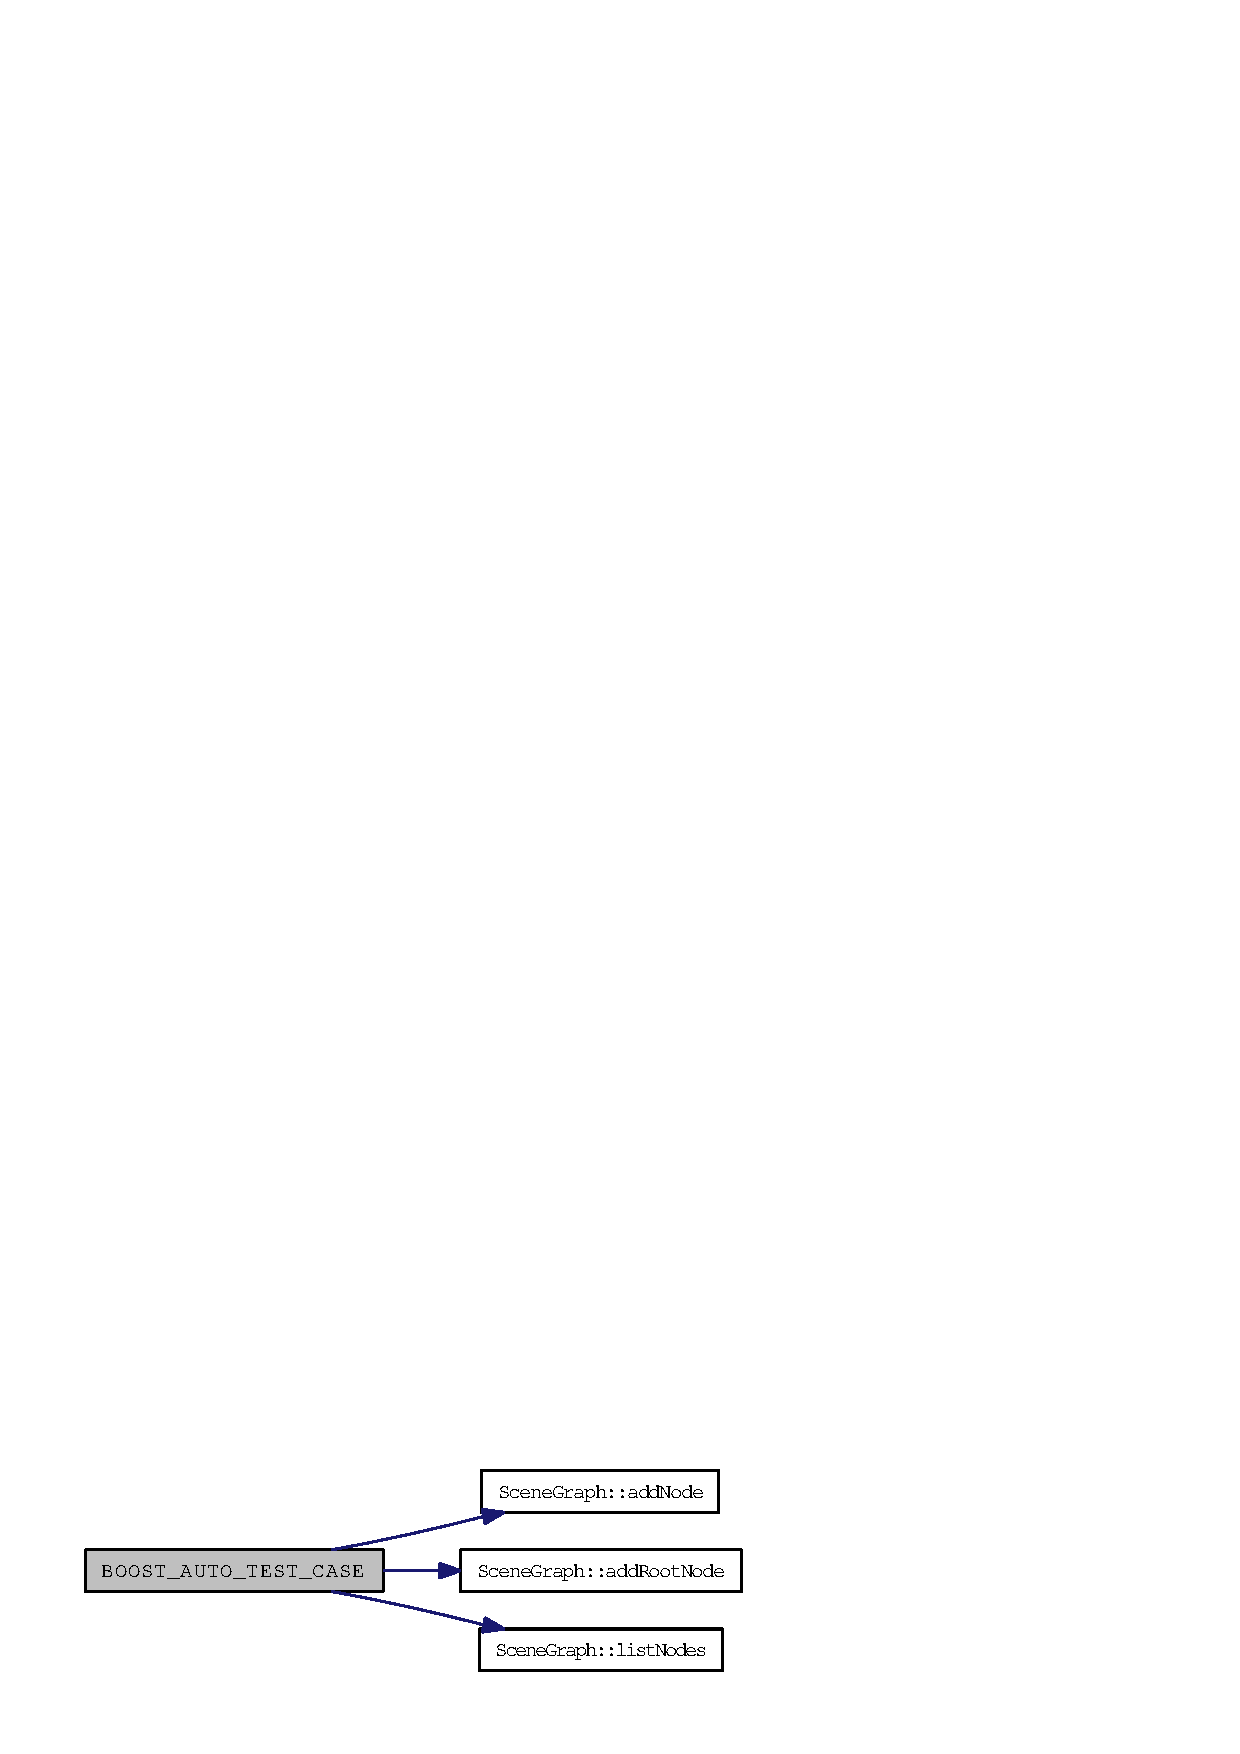
\includegraphics[width=180pt]{SceneGraphTest_8cpp_950a30b389f81084f419f5614cef9808_cgraph}
\end{center}
\end{figure}
\index{SceneGraphTest.cpp@{SceneGraphTest.cpp}!BOOST\_\-AUTO\_\-TEST\_\-CASE@{BOOST\_\-AUTO\_\-TEST\_\-CASE}}
\index{BOOST\_\-AUTO\_\-TEST\_\-CASE@{BOOST\_\-AUTO\_\-TEST\_\-CASE}!SceneGraphTest.cpp@{SceneGraphTest.cpp}}
\subsubsection{\setlength{\rightskip}{0pt plus 5cm}BOOST\_\-AUTO\_\-TEST\_\-CASE (pretty\_\-print\_\-vertices\_\-test)}\label{SceneGraphTest_8cpp_be849f12cd2b4efbcb3d9e70c340189d}




Definition at line 85 of file SceneGraphTest.cpp.

References ListGraphVisitor::getGraphList().

Here is the call graph for this function:\nopagebreak
\begin{figure}[H]
\begin{center}
\leavevmode
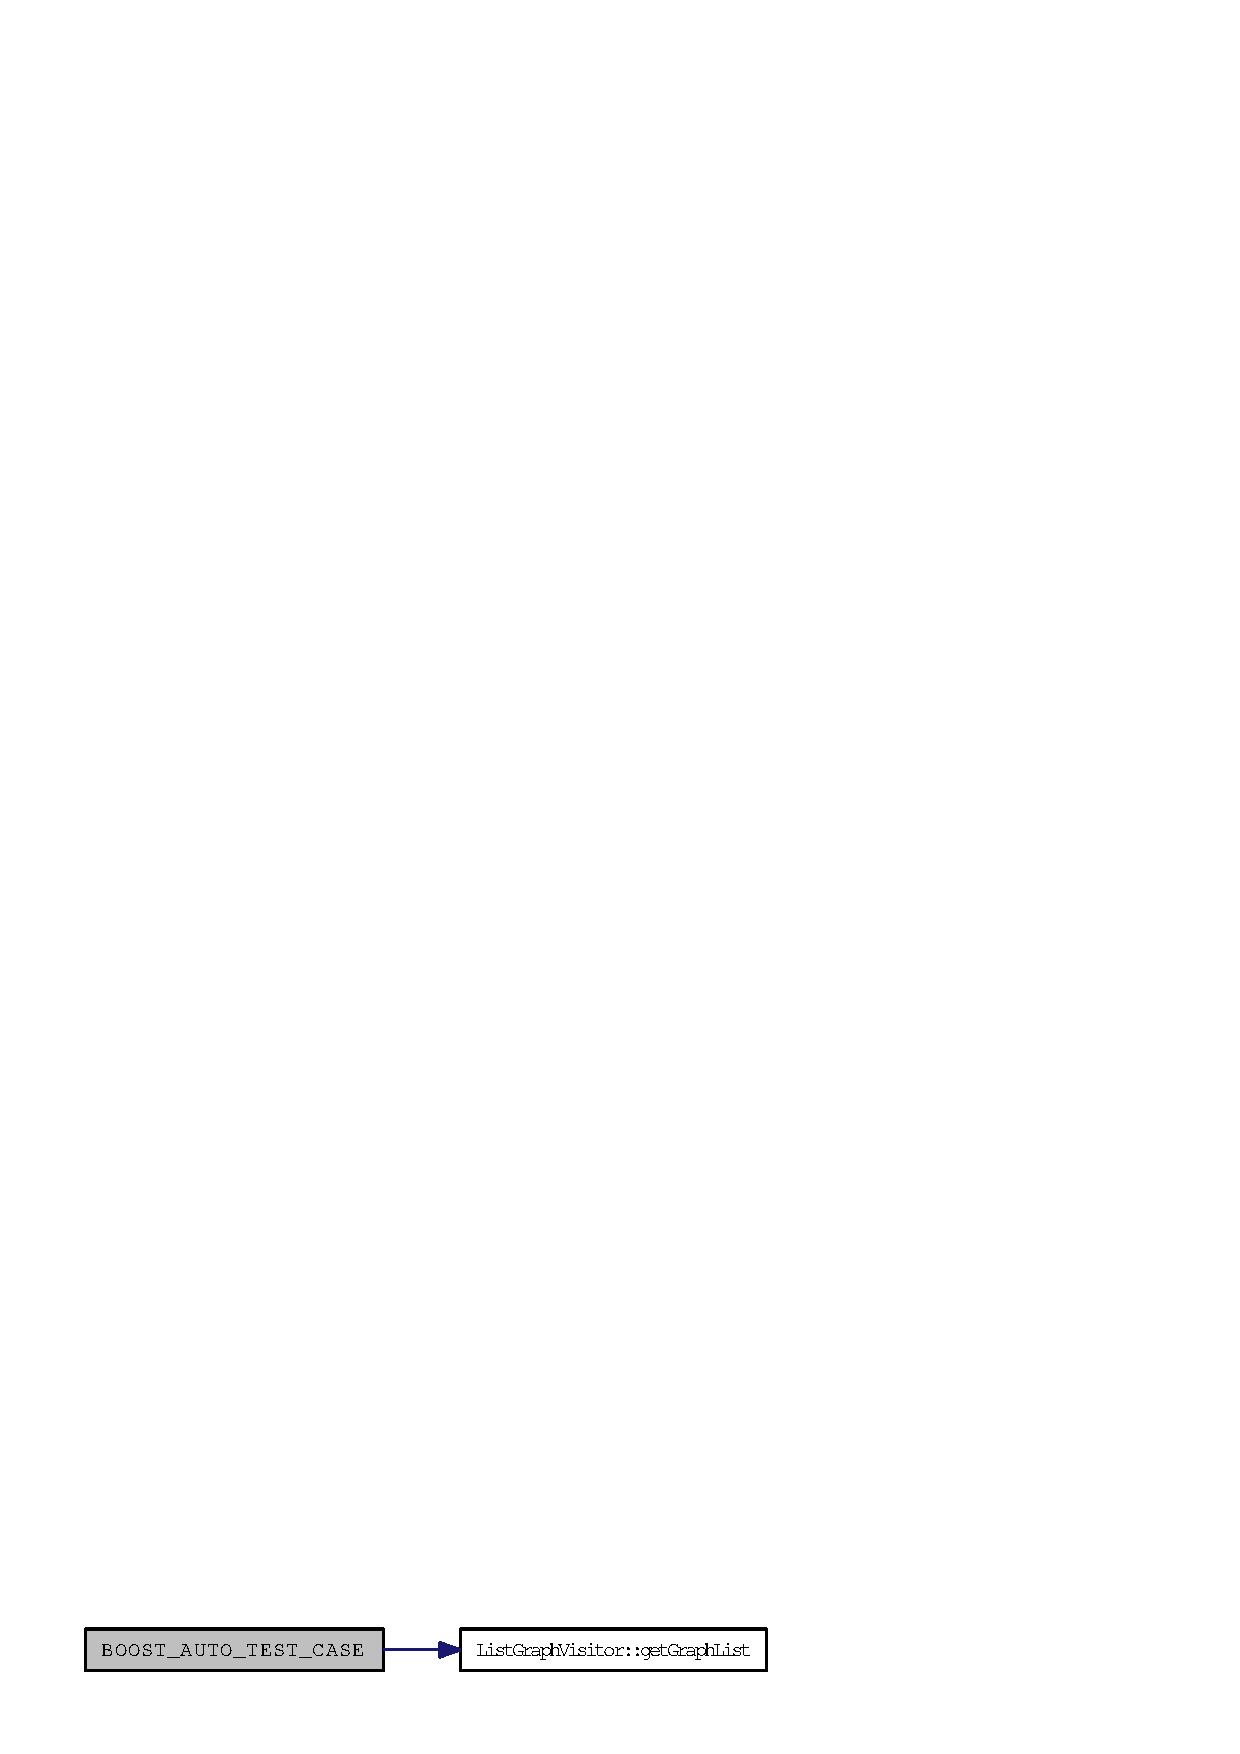
\includegraphics[width=186pt]{SceneGraphTest_8cpp_be849f12cd2b4efbcb3d9e70c340189d_cgraph}
\end{center}
\end{figure}
\index{SceneGraphTest.cpp@{SceneGraphTest.cpp}!BOOST\_\-AUTO\_\-TEST\_\-CASE@{BOOST\_\-AUTO\_\-TEST\_\-CASE}}
\index{BOOST\_\-AUTO\_\-TEST\_\-CASE@{BOOST\_\-AUTO\_\-TEST\_\-CASE}!SceneGraphTest.cpp@{SceneGraphTest.cpp}}
\subsubsection{\setlength{\rightskip}{0pt plus 5cm}BOOST\_\-AUTO\_\-TEST\_\-CASE (write\_\-dot\_\-test)}\label{SceneGraphTest_8cpp_1552d87c5d441210b23d3a67d4d83568}




Definition at line 122 of file SceneGraphTest.cpp.